\chapter[Metodologia]{Metodologia}

\label{chap:metodologia}

Neste capítulo, serão apresentados detalhes da metodologia aplicada no desenvolvimento teórico e prático do trabalho. Neste sentido, as atividades de pesquisa são classificadas conforme a abordagem, natureza, objetivos e procedimentos (seção \ref{sec:met_pesquisa}). Além disso, é definida a sequência de atividades realizadas neste trabalho de conclusão de curso (seção \ref{sec:fluxo_atividade}), detalhando aspectos metodológicos adotados no desenvolvimento do \textit{software} (seção \ref{sec:metodologia_desenvolvimento}), e na análise dos resultados obtidos (seção \ref{sec:meto_analise_resultado}). Na sequência, constam os cronogramas de atividades (seção \ref{sec:cronograma_met}), tanto para o escopo de atividades do TCC 1, quanto para o escopo de \textit{atividades} do TCC 2. Por fim, tem-se o Resumo do Capítulo (seção \ref{sec:resumo_metodologia}).

\section{Metodologia de Pesquisa}
\label{sec:met_pesquisa}
De acordo com \citeauthoronline{gerhardt2009metodos} (\citeyear{gerhardt2009metodos}), a Metodologia pode ser classificada como o estudo da organização, dos caminhos a serem trilhados, para se realizar uma pesquisa ou um estudo, ou para produzir ciência. Já a pesquisa científica, refere-se ao resultado de “um inquérito ou exame minucioso, realizado para resolver um problema, recorrendo a procedimentos científicos” \cite{gerhardt2009metodos}.

A partir das definições de \citeauthoronline{gerhardt2009metodos} (\citeyear{gerhardt2009metodos}), esta seção visa categorizar a pesquisa deste trabalho quanto à abordagem, à natureza, aos objetivos e aos procedimentos.

\subsection{Abordagem da Pesquisa}
As pesquisas utilizadas neste trabalho podem ser classificadas como Qualitativas e Quantitativas. A pesquisa qualitativa visa obter uma compreensão mais profunda de um grupo social, de uma organização, entre outros. Portanto, a pesquisa qualitativa, preocupa-se com aspectos da realidade que não podem ser quantificados, concentrando-se em compreender e explicar a dinâmica das relações sociais. Já a pesquisa quantitativa centra-se na objetividade, tendo o objetivo de enfatizar o raciocínio dedutivo, as regras da lógica e as propriedades mensuráveis da experiência humana \cite{gerhardt2009metodos}. No caso do presente trabalho, pretende-se coletar métricas qualitativas, mais associadas à Satisfação do Usuário quanto ao uso e a pertinência da ferramenta \textit{iFlow}, bem como métricas quantitativas, mais associadas, por exemplo, ao desempenho da ferramenta. Uma típica métrica quantitativa, de interesse deste trabalho, seria a taxa de defeitos encontrados, aferida contando a quantidade de ocorrências desses defeitos, por exemplo, no MVP gerado pela ferramenta.

\subsection{Natureza da Pesquisa}
A pesquisa deste trabalho pode ser classificada como Aplicada. A pesquisa aplicada visa produzir conhecimento para aplicação prática, de modo a resolver problemas específicos. Por outro lado, a pesquisa básica visa gerar conhecimentos novos, sem aplicação prática prevista \cite{gerhardt2009metodos}. O viés aplicado do trabalho é bastante sensível, dado que a ideia é prover uma ferramenta, para um público alvo, visando mitigar problemas bem específicos do domínio de uma área de interesse da Engenharia de \textit{Software}, no caso, a Engenharia de Requisitos. Adicionalmente, e ainda corroborando com a definição de uma pesquisa aplicada, a ferramenta pretende automatizar algumas atividades, e gerar um MVP.

\subsection{Objetivos da Pesquisa}
Como objetivo, a presente pesquisa classifica-se como Exploratória. A pesquisa exploratória consiste em proporcionar maior familiaridade com o problema, visando torná-lo mais explícito ou formular hipóteses \cite{gil2002elaborar}. Nesse sentido, o trabalho compreende, a partir da identificação de preocupações inerentes à área de Engenharia de Requisitos, explorar soluções que mitiguem, ao menos, tais preocupações, procurando contribuir de alguma forma com o sucesso do \textit{software} produzido, e considerando as boas práticas acordadas na literatura especializada.

\subsection{Procedimentos}
A pesquisa deste trabalho pode ser classificada como Bibliográfica e Pesquisa-Ação. A pesquisa bibliográfica é realizada a partir de um acervo de referências teóricas analisadas e publicadas por meios escritos e tecnológicos, como livros, artigos científicos, \textit{sites}, entre outros. A pesquisa-ação pressupõe a participação planejada do pesquisador na situação problemática a ser investigada, visando diagnosticar um determinado problema sobre uma dada situação, para chegar em um resultado prático \cite{gil2002elaborar}. Neste trabalho, buscou-se realizar um levantamento bibliográfico, mais bem-apresentado na seção \ref{sec:metodologia_desenvolvimento} visando acordar boas práticas e preocupações da área de Engenharia de Requisitos, ambos abordados na ferramenta \textit{iFlow}. Além disso, no intuito de analisar os resultados obtidos, em simultâneo, permitir evoluções na ferramenta com base nesses \textit{feedbacks}, pretende-se usar pesquisa-ação, conforme acordado na seção \ref{sec:meto_analise_resultado}.

\section{Fluxo de Atividades}

\label{sec:fluxo_atividade}
    
Para adequada condução deste trabalho, foram seguidas algumas etapas. Visando melhorar a visualização e evidenciar essas etapas, foi elaborado o modelo, Figura 8, com base na notação \textit{BPMN}\footnote{Notação gráfica criada pelo grupo conhecido como \textit{BPMI} no ano de 2002 para representação de processos de negócio}.

\begin{figure}[H]
    \begin{center}
        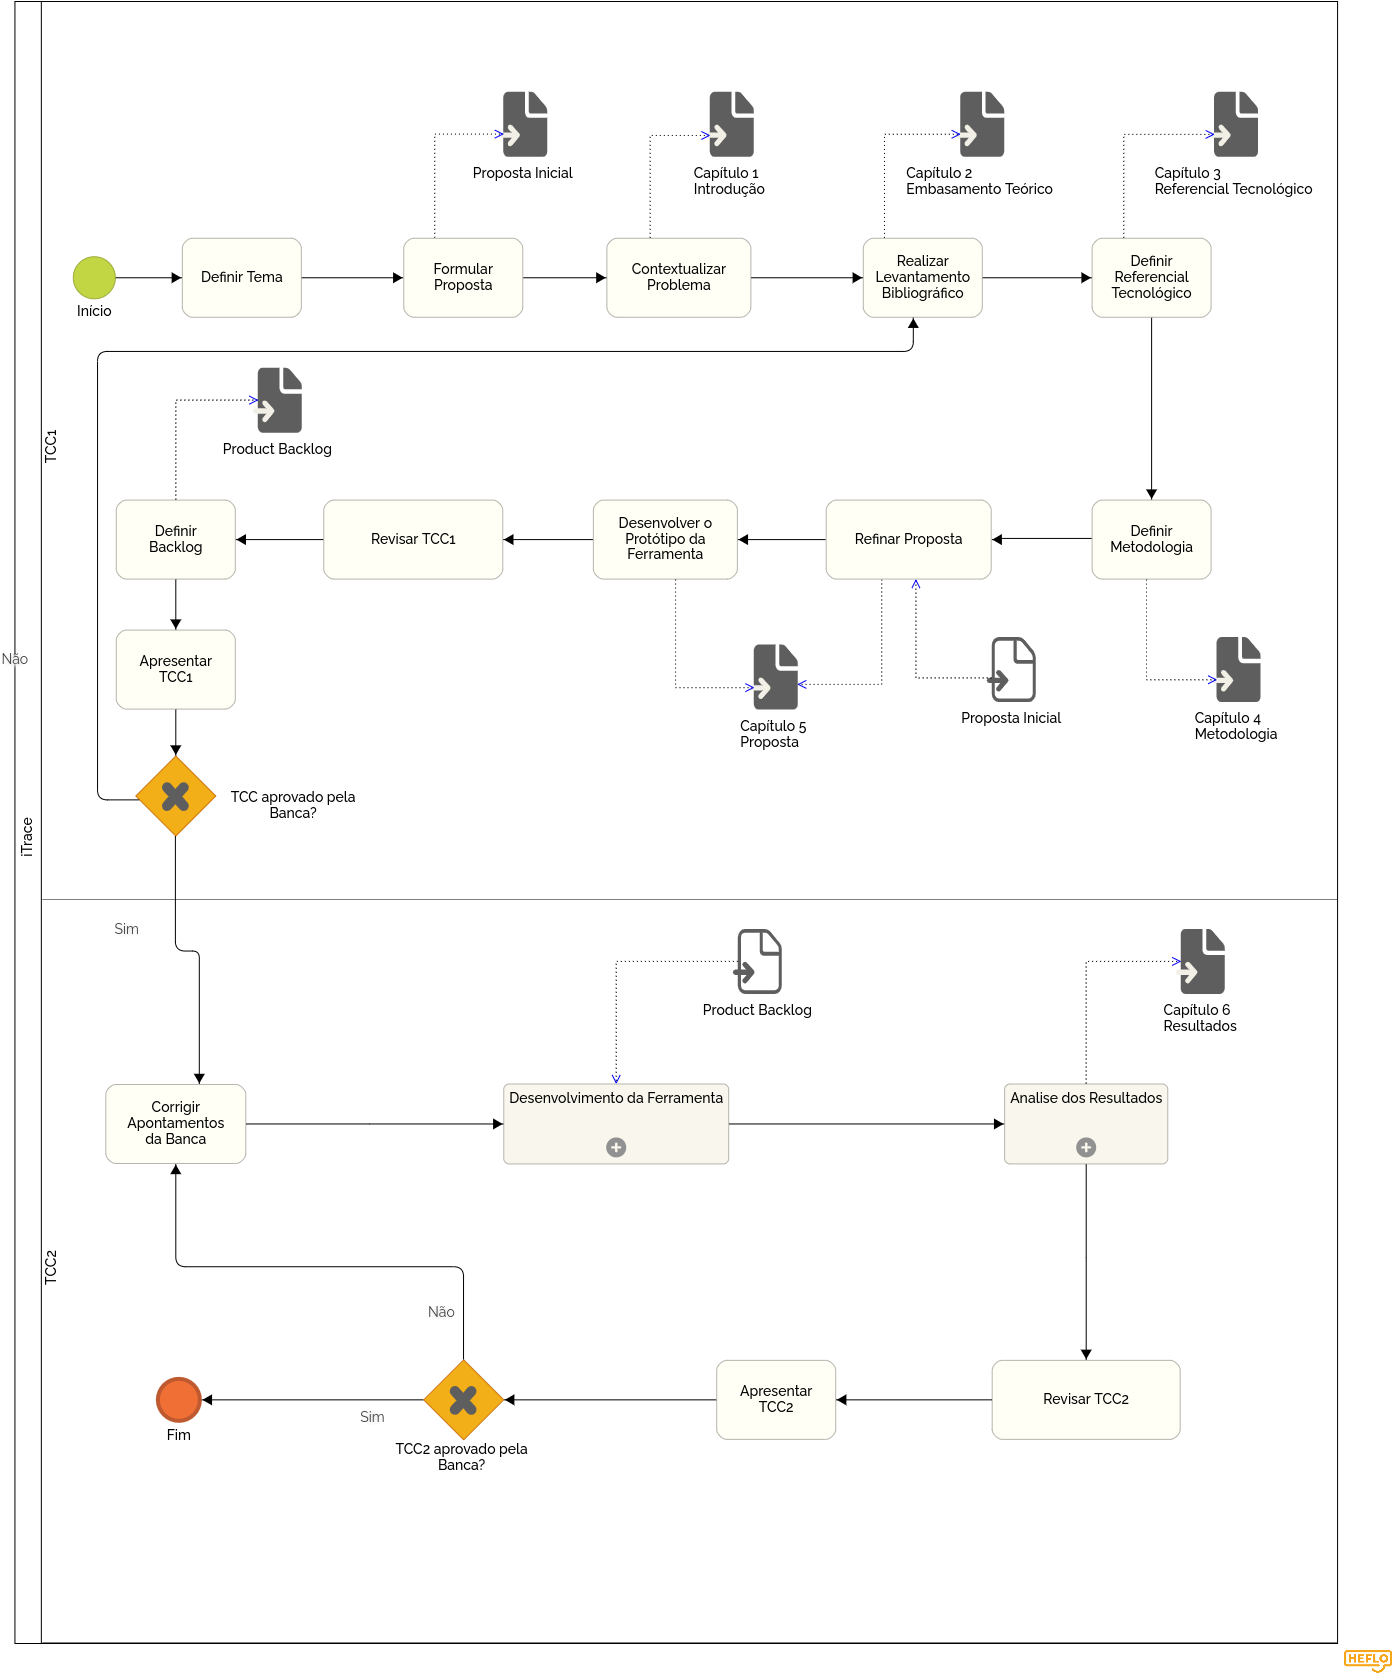
\includegraphics[scale=0.25]{figuras/Metodologia/bpmn_geral.png}
        \caption{{Fluxo de Atividades do TCC. Fonte: Autores, 2022}}
        \label{fig:bpmn_geral}
    \end{center}
\end{figure}

\begin{enumerate}
    \item \textbf{Definição do Tema}: atividade destinada à escolha do tema para o desenvolvimento do trabalho. Foram apresentados diversos temas de interesse aos orientadores, e após várias discussões, foi escolhido o tema com maior perspectiva de desenvolvimento e interesse entre as partes: a ferramenta \textit{iFlow};
    \\
    Status: Concluída;
    \item \label{item:proposta} \textbf{Formulação da Proposta}: atividade que visa o fechamento de escopo, bem como contextualizar; identificar questões de pesquisa; estabelecer os objetivos, e conferir justificativas;
    \\
    \textit{Status}: Concluída;
    \\
    Resultado: Capítulo Introdução (\ref{chap:intro});
    \item \textbf{Contextualização do Problema}: atividade que consistiu em obter uma visão mais ampla da área de interesse deste trabalho, no caso, a Engenharia de Requisitos;
    \\
    \textit{Status}: Concluída;
    \\
    Resultado: Capítulo Introdução (\ref{chap:intro});
    \item \textbf{Revisão Bibliográfica}: atividade relevante, e que permitiu consultar bases científicas, e investigar a literatura especializada sobre a área de Engenharia de Requisitos a afins. Outros detalhes, inerentes a essa atividade, constam na seção \ref{sec:metodologia_desenvolvimento};
    \\
    \textit{Status}: Concluída;
    \\
    Resultado: Capítulo Embasamento Teórico (\ref{chap:embasamento_teorico});
    \item \textbf{Definição do Suporte Tecnológico}: atividade que compreende a definição dos apoios tecnológicos, no intuito de realizar o trabalho como um todo;
    \\
    \textit{Status}: Concluída;
    \\
    Resultado: Capítulo Referencial Tecnológico (\ref{chap:referencial_tecnologico});
    \item \textbf{Definição da Metodologia}: atividade, de suma importância, em que os autores se dedicaram ao desenho de um modelo que viabilizasse a execução do trabalho na totalidade, procurando definir passos a serem cumpridos, e esquematizando-os em atividades;
    \\
    \textit{Status}: Concluída;
    \\
    Resultado: Fluxo de Atividades apresentado nesta seção (\ref{sec:fluxo_atividade});
    \item \textbf{Refinar e detalhar proposta}: atividade que visou uma maior compreensão da proposta, procurando refiná-la e detalhá-la;
    \\
    \textit{Status}: Concluída;
    \\
    Resultado: Capítulo Proposta (\ref{chap:proposta});
    \item \textbf{Desenvolvimento do Protótipo da Aplicação}: atividade destinada à elaboração de um protótipo de alta fidelidade, cujo objetivo é demonstrar, de forma mais clara, a proposta da ferramenta \textit{iFlow}. O protótipo pode ser visto ainda como uma prova de conceito, em relação à proposta, visto que acorda vários detalhamentos em termos de funcionalidades e fluxos pretendidos na ferramenta;
    \\
    \textit{Status}: Concluída;
    \\
    Resultado: Capítulo Proposta (\ref{chap:proposta});
    \item \textbf{Revisão e refinamento sistemático do TCC 1}: atividade que procura revisar cada aspecto do TCC, incluindo escrita da monografia, e elaboração de artefatos inerentes ao escopo de trabalho do TCC 1. A revisão usa iterações, tanto entre os autores, quanto dos autores com os orientadores;
    \\
    \textit{Status}: Concluída;
    \\
    Resultados: própria Monografia e artefatos em geral;
    \item \label{item:revision} \textbf{Apresentação do TCC 1}: atividade destinada à aprovação da proposta, junto à Banca Avaliadora;
    \textit{Status}: Em andamento;
    \item \textbf{Refinamento e apontamentos da Banca}: atividade que procura, com base nos \textit{feedbacks} conferidos pela Banca Avaliadora, revisar tanto a escrita da monografia, quanto a elaboração de artefatos;
    \\
    \textit{Status}: A ser realizada;
    \\
    Resultados Esperados: própria Monografia e artefatos em geral evoluídos;
    \item \textbf{Definição do \textit{Product Backlog}}: atividade relevante para iniciar o desenvolvimento da ferramenta. A ideia é elencar de forma clara e objetiva, os principais requisitos da ferramenta;
    \\
    \textit{Status}: A ser realizada;
    \\
    Resultado Esperado: \textit{Backlog} do Produto;
    \item \textbf{Desenvolvimento da Aplicação}: subprocesso que consiste no desenvolvimento da ferramenta. O detalhamento deste subprocesso encontra-se na Figura \ref{fig:bpmn_dev}. As subatividades serão explicadas na seção \ref{sec:met_dev}, na qual é definida a Metodologia de Desenvolvimento;
    \\
    % ARRUMAR AQUI DEPOIS
    \textit{Status}: A ser realizada;
    \\
    Resultado Esperado: Ferramenta \textit{iFlow};
    \item \textbf{Análise dos Resultados}: subprocesso que consiste em aplicar Pesquisa-Ação, visando coletar métricas quantitativas e qualitativas, e realizar evoluções na ferramenta, com base nessas métricas. Pretende-se, nesse processo, validar a ferramenta com apoio de testes e preenchimento de questionários junto ao público alvo. O detalhamento deste subprocesso encontra-se na Figura \ref{fig:bpmn_geral}. As subatividades serão explicadas na seção \ref{sec:meto_analise_resultado}, onde é definida a Metodologia de Análise de Resultados;
    \\
    \textit{Status}: A ser realizada;
    \\
    Resultados Esperados: Pesquisa-Ação e Ferramenta \textit{iFlow} Evoluída;
    \item \textbf{Revisão e refinamento sistemático do TCC 2}: atividade que procura revisar cada aspecto do TCC, incluindo escrita da monografia, e elaboração de artefatos inerentes ao escopo de trabalho do TCC 2. Será utilizado o mesmo processo iterativo, conduzido para o escopo do TCC 1, e
    \\
    \textit{Status}: A ser realizada;
    \\
    Resultados Esperados: Monografia e artefatos em geral, em suas versões finais;
    \item \textbf{Apresentação do TCC 2}: atividade destinada à aprovação do trabalho na totalidade, junto à Banca Avaliadora;
    \\
    \textit{Status}: A ser realizada;
\end{enumerate}

\section{Levantamento Bibliográfico}

O Levantamento Bibliográfico foi realizado de modo a buscar os problemas inerentes à Engenharia de Requisitos. Não foi desenvolvida uma \textit{string} de busca, mas o objetivo foi encontrar fontes confiáveis para o embasamento deste Trabalho de Conclusão de Curso.

Os principais autores e artigos usados tiveram como base referências usadas em disciplinas anteriores, cursadas durante a graduação. As palavras-chave utilizadas para guiar as pesquisas foram as mesmas usadas para as definições contidas no Embasamento Teórico (Capítulo \ref{chap:embasamento_teorico}), tais como: Engenharia de Requisitos, Elicitação, Modelagem, \textit{House of Quality}, entre outros.

Vale ressaltar que os termos correspondentes foram utilizados na língua inglesa para que houvesse uma maior quantidade de referências no contexto proposto. 

\section{Metodologia de Desenvolvimento}

\label{sec:metodologia_desenvolvimento}

No que tange a metodologia voltada ao desenvolvimento prático da ferramenta, por afinidade da dupla, a combinação de duas metodologias, \textit{Scrum} \& \textit{Kanban}, as quais serão adaptadas em função do perfil do trabalho.

O \textit{Scrum} é uma metodologia ágil para desenvolvimento de produtos complexos que mudam os requisitos rapidamente. O seu desenvolvimento é dado por uma série de iterações chamadas \textit{Sprint}, que no caso do nosso projeto, serão semanais. A cada \textit{Sprint} é realizada uma reunião de planejamento (\textit{Sprint Planning}) e de revisão do trabalho (\textit{Sprint Review \& Restrospective}), com foco na melhoria contínua do processo e iteração entre as pessoas. Para promover a transparência e o alinhamento do trabalho, serão utilizados dois artefatos, o \textit{Backlog} do Produto (\textit{Product Backlog}) e o \textit{Backlog} da \textit{Sprint} (\textit{Sprint Backlog}), nos quais é descrito no trabalho a ser realizado, respectivamente, no escopo do produto e no escopo da \textit{Sprint} \cite{carolipaulo2021}.

O \textit{Kanban} é uma metodologia que visa um alinhamento mais claro de uma equipe, além de dar visibilidade ao que está sendo elaborado, proporcionando um ambiente favorável à comunicação, com o menor ruído possível. Além disso, garante uma carga de trabalho adequada, considerando a capacidade produtiva da equipe. Um ponto essencial dessa metodologia é o quadro que deixa as tarefas e seus \textit{status} visíveis para todo o time, pontuando em qual parte do fluxo de trabalho cada tarefa se encontra \cite{K_Condensed}.

\subsection{Processo de Desenvolvimento}

\label{sec:met_dev}

O processo de desenvolvimento escolhido pode ser visualizado na Figura \ref{fig:bpmn_dev}, elaborado com base na notação \textit{BPMN},  a partir do detalhamento do subprocesso \textbf{Desenvolvimento da Ferramenta}, apresentado na Figura \ref{fig:bpmn_geral}, consistindo das seguintes etapas:

\begin{figure}[H]
    \begin{center}
        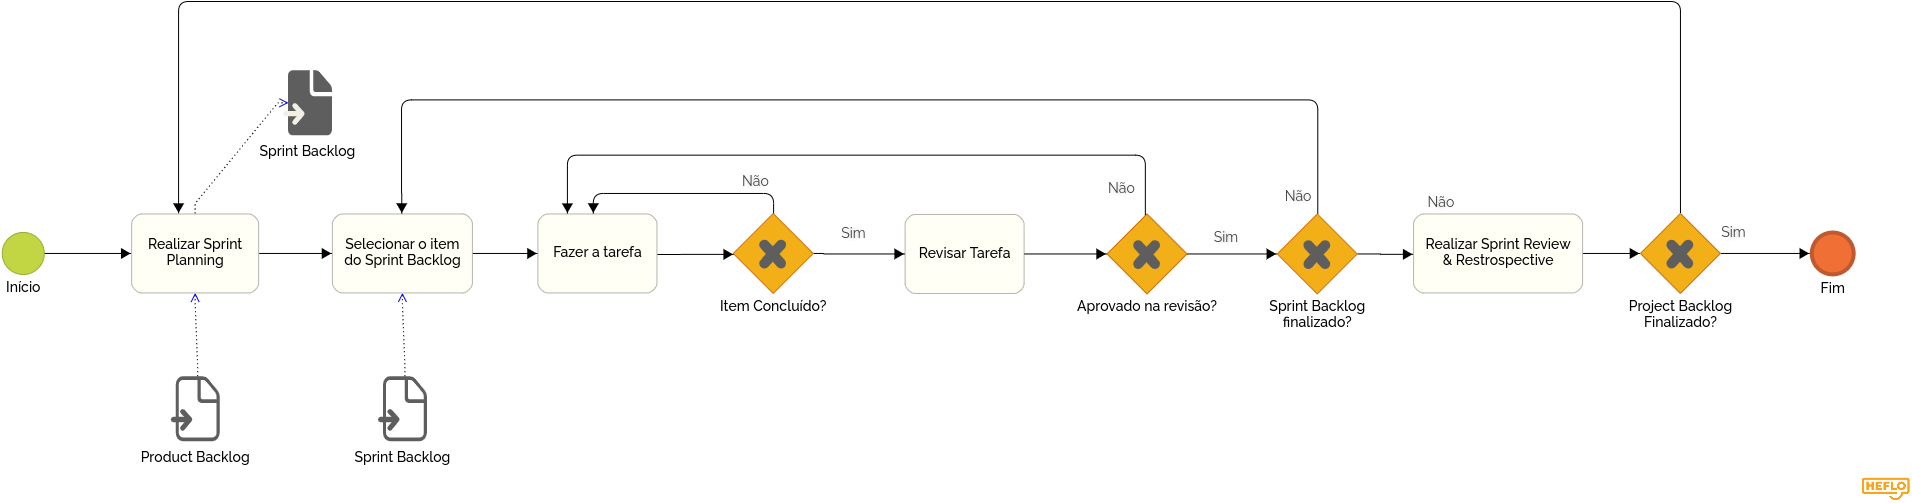
\includegraphics[scale=0.23]{figuras/Metodologia/bpmn_dev.png}
        \caption{{Fluxo de Atividades do Subprocesso Desenvolvimento da Ferramenta \textit{iFlow}. Fonte: Autores, 2022}}
        \label{fig:bpmn_dev}
    \end{center}
\end{figure}

\begin{enumerate}
    \item \textbf{\textit{Sprint Planning}}: a partir do \textit{Product Backlog}, as atividades são selecionadas consoante a sua prioridade e pontos definidos para execução da mesma. As tarefas selecionadas consideram a capacidade produtiva dos autores na \textit{Sprint} e a gestão de riscos para a entrega do produto. Ao final, é esperado o \textit{Sprint Backlog};
    \item \textbf{Selecionar o \textit{item} do \textit{Sprint Backlog}}: a partir do \textit{Sprint Backlog}, as tarefas são selecionadas para serem executadas pelos autores;
    \item \textbf{Fazer a tarefa}: consiste em desenvolver a tarefa selecionada;
    \item \textbf{Revisar tarefa}: consiste no processo de revisão por parte, dentre os autores, do membro que não atuou no desenvolvimento diretamente, para verificar se os padrões de desenvolvimento da comunidade foram seguidos, e se atende ao que foi definido no \textit{Product Backlog};
    \item \textbf{\textit{Sprint Review \& Restrospective}}: com a conclusão da \textit{Sprint}, essa atividade elenca os pontos positivos e negativos da \textit{sprint}, além de revisar as atividades entregues.
\end{enumerate}


\section{Metodologia de Análise de Resultados}

\label{sec:meto_analise_resultado}

Como definido na Seção \ref{sec:met_pesquisa}, o método orientado para o processo de análise dos resultados do trabalho será a Pesquisa-Ação. De acordo com \citeauthoronline{gil2002elaborar} (\citeyear{gil2002elaborar}), a pesquisa-ação ocorre com muitas oscilações entre as fases, determinada pela dinâmica do grupo de pesquisadores em seu relacionamento com a situação pesquisada. Além disso, a pesquisa-ação apresenta uma série de ações desordenadas no tempo, considerando os seguintes passos: a) fase exploratória; b) formulação do problema; c) construção de hipóteses; d) realização do seminário; e) seleção da amostra; f) coleta de dados; g) análise e interpretação dos dados; h) elaboração do plano de ação; e i) divulgação dos resultados.

Já conferindo uma versão adaptada do protocolo, a pesquisa-ação a ser utilizada neste trabalho será conduzida com base nas seguintes etapas:

\begin{itemize}
    \item \textbf{Coleta de dados}: nesta etapa, realiza-se a coleta de dados quantitativos por meio da ferramenta desenvolvida, e qualitativos através da interação dos usuários com a ferramenta;
    \item \textbf{Análise e interpretação dos dados}: nesta etapa, busca-se examinar os dados coletados e, em seguida, realizar a explanação dos resultados adquiridos;
    \item \textbf{Elaboração do plano de ação}: pretende-se elaborar um plano de ação que visa mitigar os problemas encontrados a partir dos dados analisados, e 
    \item \textbf{Divulgação dos resultados}: para validação, os resultados obtidos e o plano de ação definido, será validado com a banca, bem como junto ao público alvo,
    no intuito de compreender sobre as contribuições da ferramenta no escopo de atuação da mesma.
\end{itemize}

Dentre as investigações, pretende-se ter uma iteração mais voltada a testes com os \textit{stakeholders} que avaliam a experiência do usuário na ferramenta, de forma a validar se a ferramenta cumpre com os \textbf{objetivos específicos} \ref{oe_guiar_usuario} e \ref{oe_ux_facilitada}. Pretende-se também realizar testes que busquem validar se os requisitos propostos foram cumpridos e, principalmente, se o \textbf{objetivo específico} \ref{oe_mvp} foi satisfeito. Há ainda a possibilidade de realizar a coleta de métricas quantitativas, sendo assim, havendo a necessidade de pelo menos uma iteração nesse sentido.

\section{Cronogramas}

\label{sec:cronograma_met}

As Tabelas \ref{tab:cronograma_tcc1} e \ref{tab:cronograma_tcc2} apresentam os cronogramas do TCC 1 e 2, respectivamente. Nas tabelas, as atividades são descritas de acordo com suas datas de implementação, baseando-se no fluxo de atividades descrito na Seção \ref{sec:fluxo_atividade}, e considerando uma temporalidade contínua e não baseada apenas em período letivo.

\begin{table}[H]
    \centering
    \scalebox{0.9}{%
    \begin{tabular}{l*{4}{c}r}
        \hline
        Atividade & Jan/2022 & Fev/2022 & Mar/2022 & Abr/2022 \\
        \hline
        Definição do Tema & X & & & \\
        Formulação da Proposta & & X & & \\
        Contextualização do Problema & & X & & \\
        Revisão Bibliográfica & & & X & \\
        Definição de Suporte Tecnológico & & & X & \\
        Definição da Metodologia & & & X & \\
        Refinar e Detalhar Proposta & & & & X \\
        Desenvolvimento do Protótipo da Aplicação & & & & X \\
        Revisão e Refinamento sistemático do TCC & & & & X \\
        Apresentação do TCC 1 & & & & X \\
        \hline
    \end{tabular}}
    \caption{Cronograma de Atividades do TCC 1}
    \label{tab:cronograma_tcc1}
\end{table}

\begin{table}[H]
    \centering
    \scalebox{0.8}{%
    \begin{tabular}{l*{5}{c}r}
        \hline
        Atividade & Mai/2022 & Jun/2022 & Jul/2022 & Ago/2022 & Set/2022 \\
        \hline
        Refinamento e apontamentos da Banca & X & & & & \\
        Definição do \textit{Product Backlog} & X & & & & \\
        Desenvolvimento da Aplicação & X & X & X & X & \\
        Análise dos Resultados & & & & X & X \\
        Revisão e refinamento sistemático do TCC & & & & & X \\
        Apresentação do TCC 2 & & & & & X \\
        \hline
    \end{tabular}}
    \caption{Cronograma de Atividades do TCC 2}
    \label{tab:cronograma_tcc2}
\end{table}

\section{Resumo do Capítulo}
\label{sec:resumo_metodologia}
Neste capítulo, foram apresentadas as escolhas metodológicas definidas para o desenvolvimento deste Trabalho de Conclusão de Curso. Desta forma, foram evidenciadas as metodologias da fase de pesquisa, de desenvolvimento da proposta, e de análise dos resultados, a fim de identificar e categorizar os pontos mais importantes em cada uma delas. A seguir, visando retratar as etapas de desenvolvimento do trabalho, foram apresentados os fluxos de atividades que orientam o desenvolvimento do trabalho com as respectivas descrições correspondentes das atividades ilustradas nesses fluxos. Por fim, os cronogramas das duas fases de realização do trabalho (TCC 1 e TCC 2) foram apresentados.